\item Uma atração de parque de diversões consiste de uma carro que está fixo ao cabo $OA$. O carro gira em uma trajetória circular horizontal e atinge velocidade $v_{1}=\SI{1.2}{\meter/\second}$, quando $r=\SI{3.6}{\meter}$. O cabo é então recolhido a uma taxa constante de \SI{.15}{\meter/\second}. Determine a velocidade do carro em 3 segundos.

\import{sections/answers/}{answer-8}

\vspace{-1cm}
\begin{flushright}
	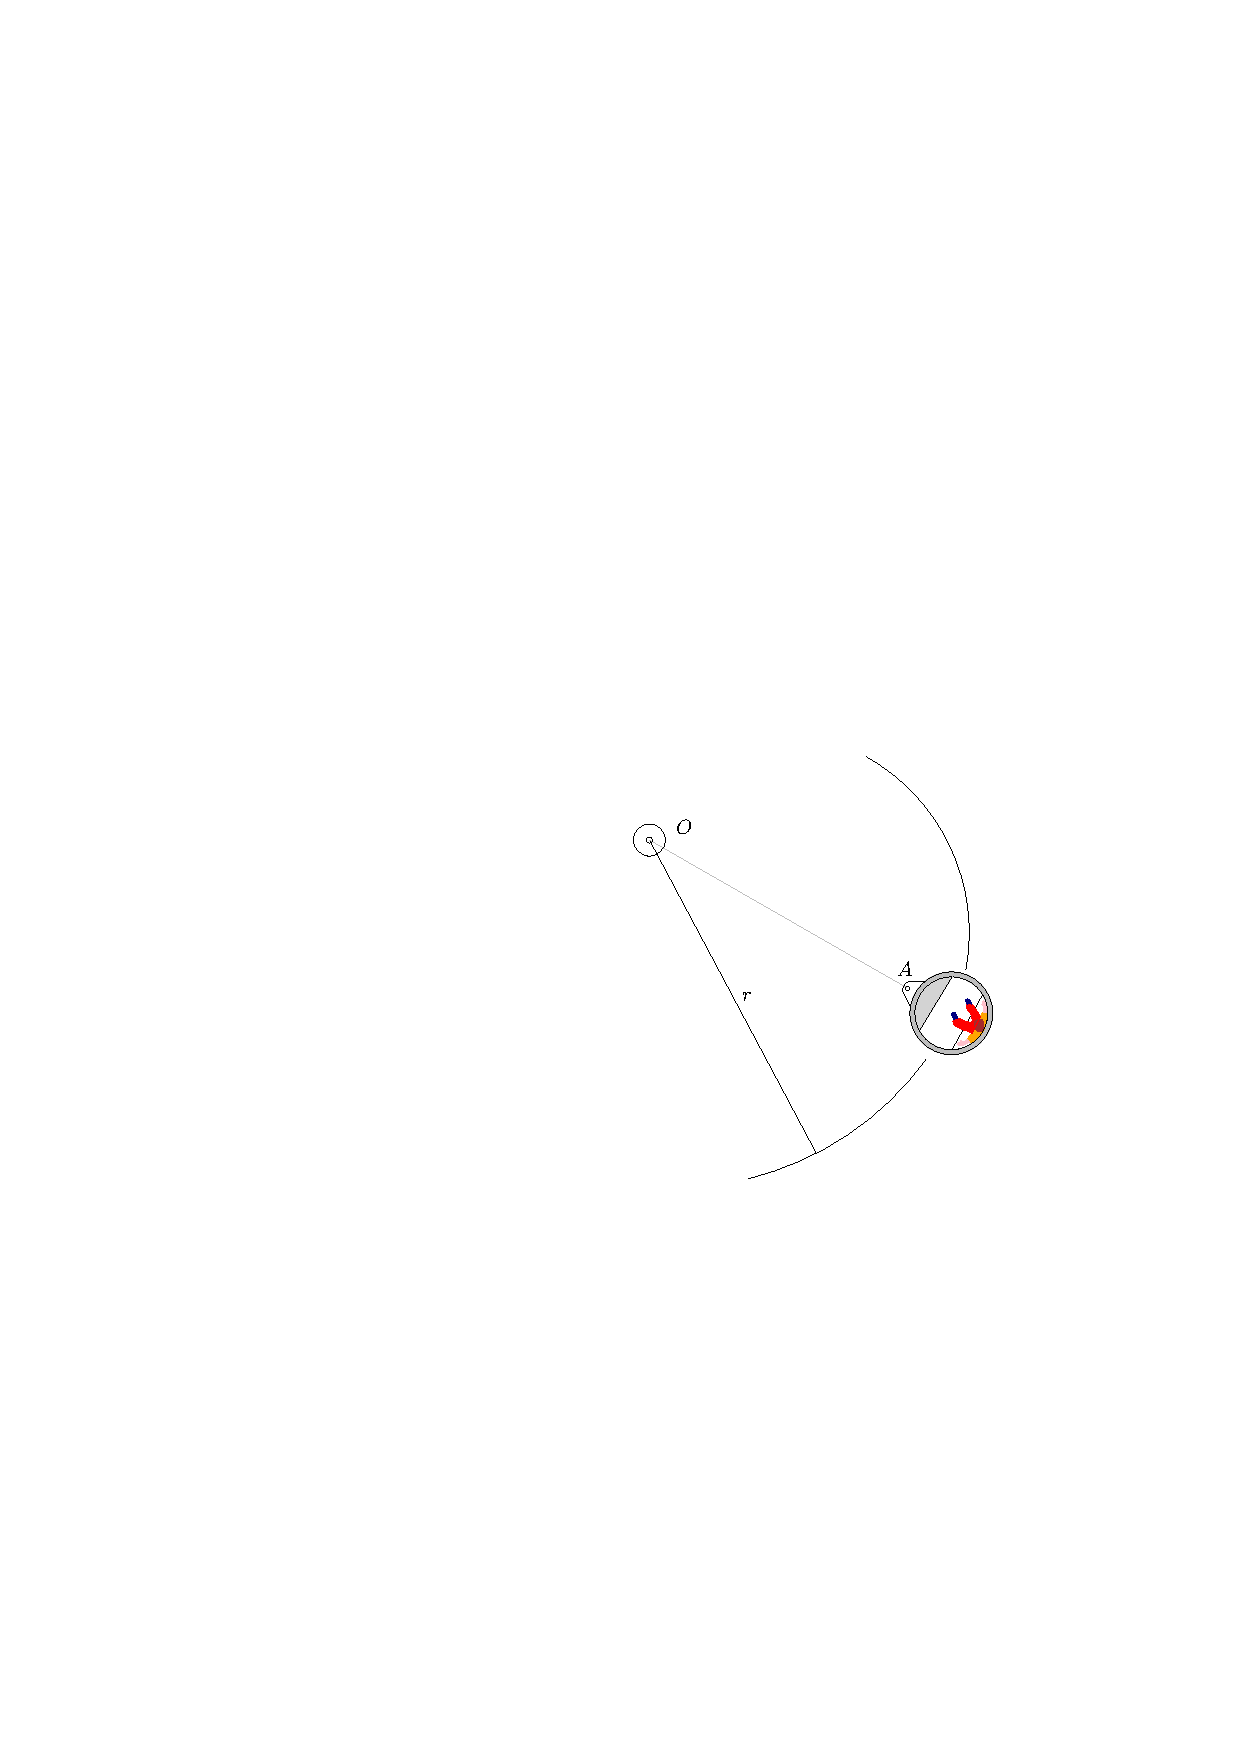
\includegraphics[scale=1.3]{images/draw_8}
\end{flushright}